\documentclass[11pt, a4paper]{article}

\usepackage{graphicx}
\usepackage[a4paper,top=3cm,bottom=2cm,left=2cm,right=2cm,marginparwidth=1.75cm]{geometry}
\usepackage[english]{babel}
\usepackage[utf8x]{inputenc}
\usepackage{subfig}
\usepackage{amsmath}
\usepackage{amssymb}
\usepackage{mhchem}
\usepackage{hyperref}
\usepackage{tikz}

\graphicspath{ {./images} }
\newcommand*{\qed}{\hfill\ensuremath{\quad\square}}%
\newcommand*{\rad}{\ensuremath{\,\text{rad}}}
\newcommand*{\R}{\ensuremath{\mathbb{R}}}

\makeatletter
\renewcommand*\env@matrix[1][*\c@MaxMatrixCols c]{%
  \hskip -\arraycolsep
  \let\@ifnextchar\new@ifnextchar
  \array{#1}}
\makeatother

\newtheorem{theorem}{Theorem}

%------------------------------------------------
%Templates for images and figures
% \begin{figure}[h]
%   \centering
%   \subfloat[caption 1]{{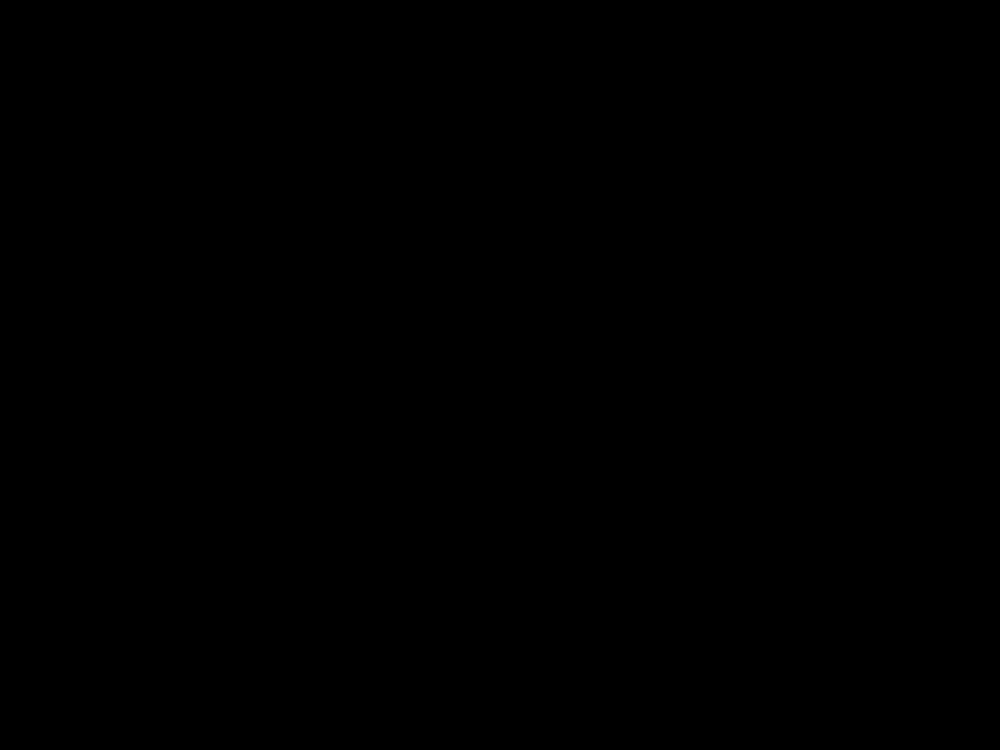
\includegraphics[width=30mm]{images/placeholder.png}}}%
%   \qquad
%   \subfloat[caption 2]{{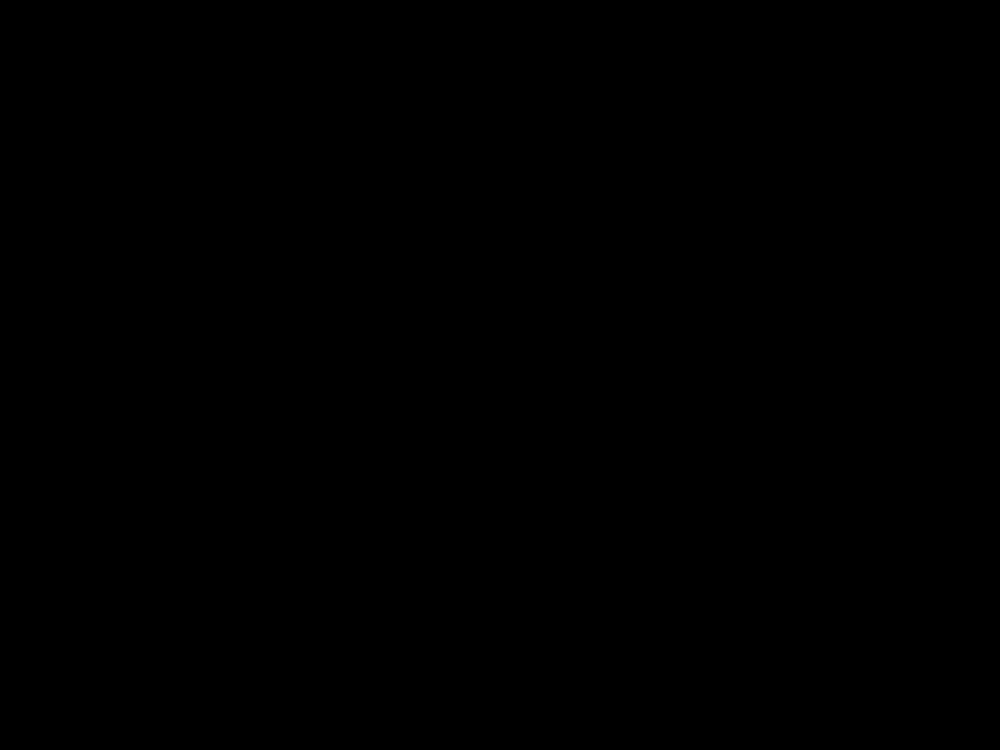
\includegraphics[width=30mm]{images/placeholder.png}}}%
%   \caption{Description}
% \end{figure}

% \begin{figure}[h]
%   \centerline{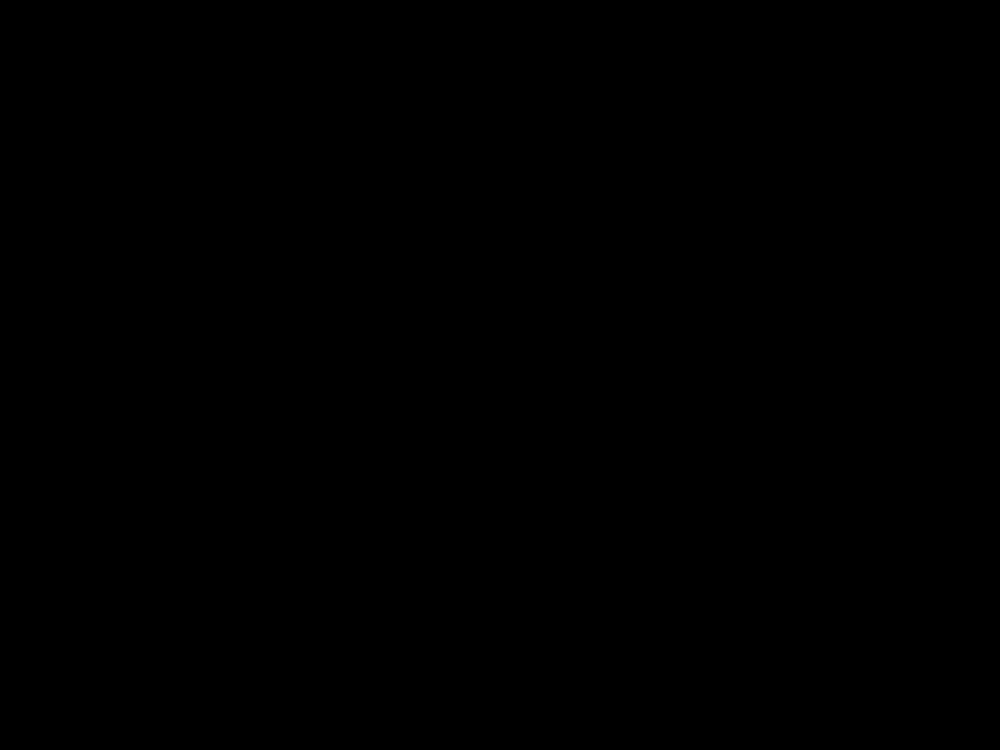
\includegraphics[width=50mm]{images/placeholder.png}}
%   \caption{Description}
% \end{figure}

%Template for a simple table 
%\begin{table}[h]
%   \caption{Description} %title of the table
%   \centering % centering table
%   \begin{tabular}{l rr} % creating three columns
%     \hline\hline %inserting double-line
%     & & \\ [0.5ex] % Insert half line vertical spacing
%     \hline % inserts single-line
%     & & \\ 
%     & & \\
%     & & \\
%     & & \\
%   \hline % inserts single-line
%   \end{tabular}
%   \label{tab:hresult}
% \end{table}
%-----------------------------------------------

\begin{document}
\setcounter{section}{7}
\setcounter{equation}{0}

\section{Thermofluid lecture 8: Non stationary control volumes and example systems}

\subsection{Non-stationary control volumes}
Recall the law of conservation of mass as it applies to an open system:
\begin{equation}
  \frac{dm_{CV}}{dt} = \sum_{in} \dot{m}_{in} - \sum_{out} \dot{m}_{out}
\end{equation}
When analyzing stationary control volumes we set the $\frac{dm_{CV}}{dt}$ term to $0$. For situations where the control volume is not volume setting this term to $0$ doesn't hold anymore. Instead we integrate both sides with respect to time:
\begin{equation*}
  \int_{0}^{t} \frac{dm_{CV}}{dt}\,dt = \int_{0}^{t} \sum_{in} \dot{m}_{in} \, dt - \int_{0}^{t} \sum_{out} \dot{m}_{out} \, dt
\end{equation*}
This equation then becomes:
\begin{equation}
  \label{eqn:consv_open_system}
  m_{CV}(t) - m_{CV}(0) = \sum_{in} m_{in} - \sum_{out} m_{out}
\end{equation}
Where equation \ref{eqn:consv_open_system} represents the conservation of mass law as it is applied to an open system with non-stationary control volume. This same idea also holds when considering the energy balance of the control volume. Recall the equation for energy balance of an open system with stationary control volume:
\begin{equation}
  \label{eqn:consv_energy}
  \frac{dE_{CV}}{dt} = \dot{Q}_{CV} - \dot{W}_{CV} + \sum_{in} \dot{m}_{in} \theta_{in} - \sum_{out} \dot{m}_{out} \theta_{out}
\end{equation}
Since the terms for $\Delta PE$ and $\Delta KE$ are often much smaller compared to internal energy we can approximate that $\frac{dE_{CV}}{dt} = \frac{dU_{CV}}{dt}$. When integrating equation \ref{eqn:consv_energy} with respect to time we end up with:
\begin{equation*}
  \int_{0}^{t} \frac{dE_{CV}}{dt} \,dt = \int_{0}^{t} \dot{Q}_{CV} \, dt - \int_{0}^{t} \dot{W}_{CV} \, dt + \int_{0}^{t} \sum_{in} \dot{m}_{in} \theta_{in} \, dt - \int_{0}^{t} \sum_{out} \dot{m}_{out} \theta_{out} \, dt
\end{equation*}
This integrates to the following equation:
\begin{equation}
  U_{CV}(t) - U_{CV}(0) = Q_{CV} - W_{CV} + \sum_{in} m_{in} \theta_{in} - \sum_{out} m_{out} \theta_{out}  
\end{equation}


\subsection{TODO}
pass


\end{document}